\section{Spline Interpolation}

Given a set of measurement points with arguments $x_0,x_1,\ldots,x_n$.

\makebox[\columnwidth]{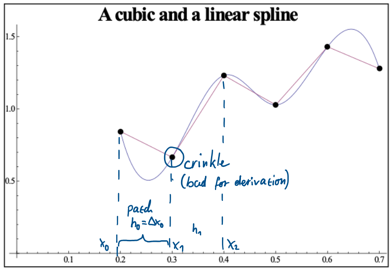
\includegraphics[width=0.6\columnwidth]{images/splines}}

The splines have to be a continuous curve ($C^0$) and often fulfill a smoothness condition
($C^1$ = cont. derivative, $C^2$ = cont. second derivative, ...).
Typical situation is that we seek patching polynomials of degree $d$ which must be a $C^{d-1}$ curve.
It is assumed that $n > d-1$ and gives a total of $n(d-1) + 2n - (d-1) = n(d+1) - (d-1)$ conditions.

\subsection{Cubic Splines}

For degree $d = 3$ and $i=0,1,\ldots,n-1$ we define a cubic polynomial
\begin{snugshade*}
    belonging to patch $[x_i,x_{i+1}]$ ($h=x_{i+1}-x_i = \Delta x_i$):
    \begin{align*}
        S_i(x) = a_i + b_i(x-x_i) + c_i(x-x_i)^2 + d_i(x-x_i)^3
    \end{align*}
\end{snugshade*}

To determine the coefficients, the following equations can be used:

\begin{snugshade*}
    \textbf{For $\mathbf{a_i}$:}
    \begin{align}
        \label{spline-a}
        a_i = y_i\ (i=0,\ldots,n-1)
    \end{align}

    \textbf{For $\mathbf{b_i}$:}
    \begin{align}
        \label{spline-b}
        b_{i-1}=\frac{a_i-a_{i-1}}{h_{i-1}}-\frac{2c_{i-1}+c_i}{3}h_{i-1}\ (i=1,\ldots,n-1)
    \end{align}
    while the last one is
    \begin{align}
        \label{spline-bn}
        b_{n-1} = \frac{y_n - a_{n-1}}{h_{n-1}}-c_{n-1}h_{n-1}-d_{n-1}h_{n-1}^2
    \end{align}

    \textbf{For $\mathbf{c_i}$ coefficients:} $((n-2)\times n)$ linear system
    (underdetermined $\Rightarrow$ many solutions)
    \begin{align*}
        \ & \resizebox{\columnwidth}{!}{$
        \begin{bmatrix}
            h_0 & 2(h_0 + h_1) & h_1          & 0       & \hdots               & 0       \\
            0   & h_1          & 2(h_1 + h_2) & h_2     & \hdots               & 0       \\
            0   & 0            & \ddots       & \ddots  & \ddots               & \vdots  \\
            0   & 0            & 0            & h_{n-3} & 2(h_{n-3} + h_{n-2}) & h_{n-2}
        \end{bmatrix}\cdot
        \begin{bmatrix}
            c_0    \\
            c_1    \\
            c_2    \\
            \vdots \\
            c_{n-1}
        \end{bmatrix}
        $} \\
        \ & =
        \begin{bmatrix}
            \vdots                                                                \\
            3\left(\frac{y_{i+1} - y_i}{h_i}-\frac{y_i - y_{i-1}}{h_{i-1}}\right) \\
            \vdots
        \end{bmatrix}_{i=1,\ldots,n-2}
    \end{align*}

    \textbf{For $\mathbf{d_i}$:}
    \begin{align}
        \label{spline-d}
        d_{i-1} = \frac{c_i - c_{i-1}}{3h_{i-1}}
    \end{align}
\end{snugshade*}

\subsubsection{Natural Cubic Splines}
Fulfils the boundary condition $S''(x_0)=S''(x_n)=0$ and minimises the mean total curvature
$\int_{x_0}^{x_n}|f''(x)|^2\ dx$.
The tri-diagonal system of equations takes the regular form ($n-1$ equations for $n-1$ coeff.):
\begin{align*}
    \ & \resizebox{\columnwidth}{!}{$
    \begin{bmatrix}
        2(h_0 + h_1) & h_1          & 0       & \hdots               & 0                    \\
        h_1          & 2(h_1 + h_2) & h_2     & \hdots               & 0                    \\
        0            & 0            & \ddots  & \ddots               & \vdots               \\
        0            & 0            & h_{n-3} & 2(h_{n-3} + h_{n-2}) & h_{n-2}              \\
        0            & 0            & 0       & h_{n-2}              & 2(h_{n-2} + h_{n-1})
    \end{bmatrix}\cdot
    \begin{bmatrix}
        c_0     \\
        c_1     \\
        \vdots  \\
        c_{n-2} \\
        c_{n-1}
    \end{bmatrix}
    $} \\
    \ & =
    \begin{bmatrix}
        \vdots                                                                \\
        3\left(\frac{y_{i+1} - y_i}{h_i}-\frac{y_i - y_{i-1}}{h_{i-1}}\right) \\
        \vdots
    \end{bmatrix}_{i=1,\ldots,n-1}
\end{align*}

The $d$-coefficients take the form as described in (\ref{spline-d}) with
\begin{align}
    \label{spline-dn}
    d_{n-1} = -\frac{c_{n-1}}{3h_{n-1}}
\end{align}
and the $b$-coefficients as described in (\ref{spline-b}) and (\ref{spline-bn}).

\subsubsection{``Clamped''/Complete Cubic Splines}

These splines satisfy a first order derivative condition on the boundary arguments:
\begin{align*}
    S'(x_0)=y'_0\text{ and }S'(x_n)=y'_n
\end{align*}

The linear system for the $c$-coefficients:
\makebox[\columnwidth]{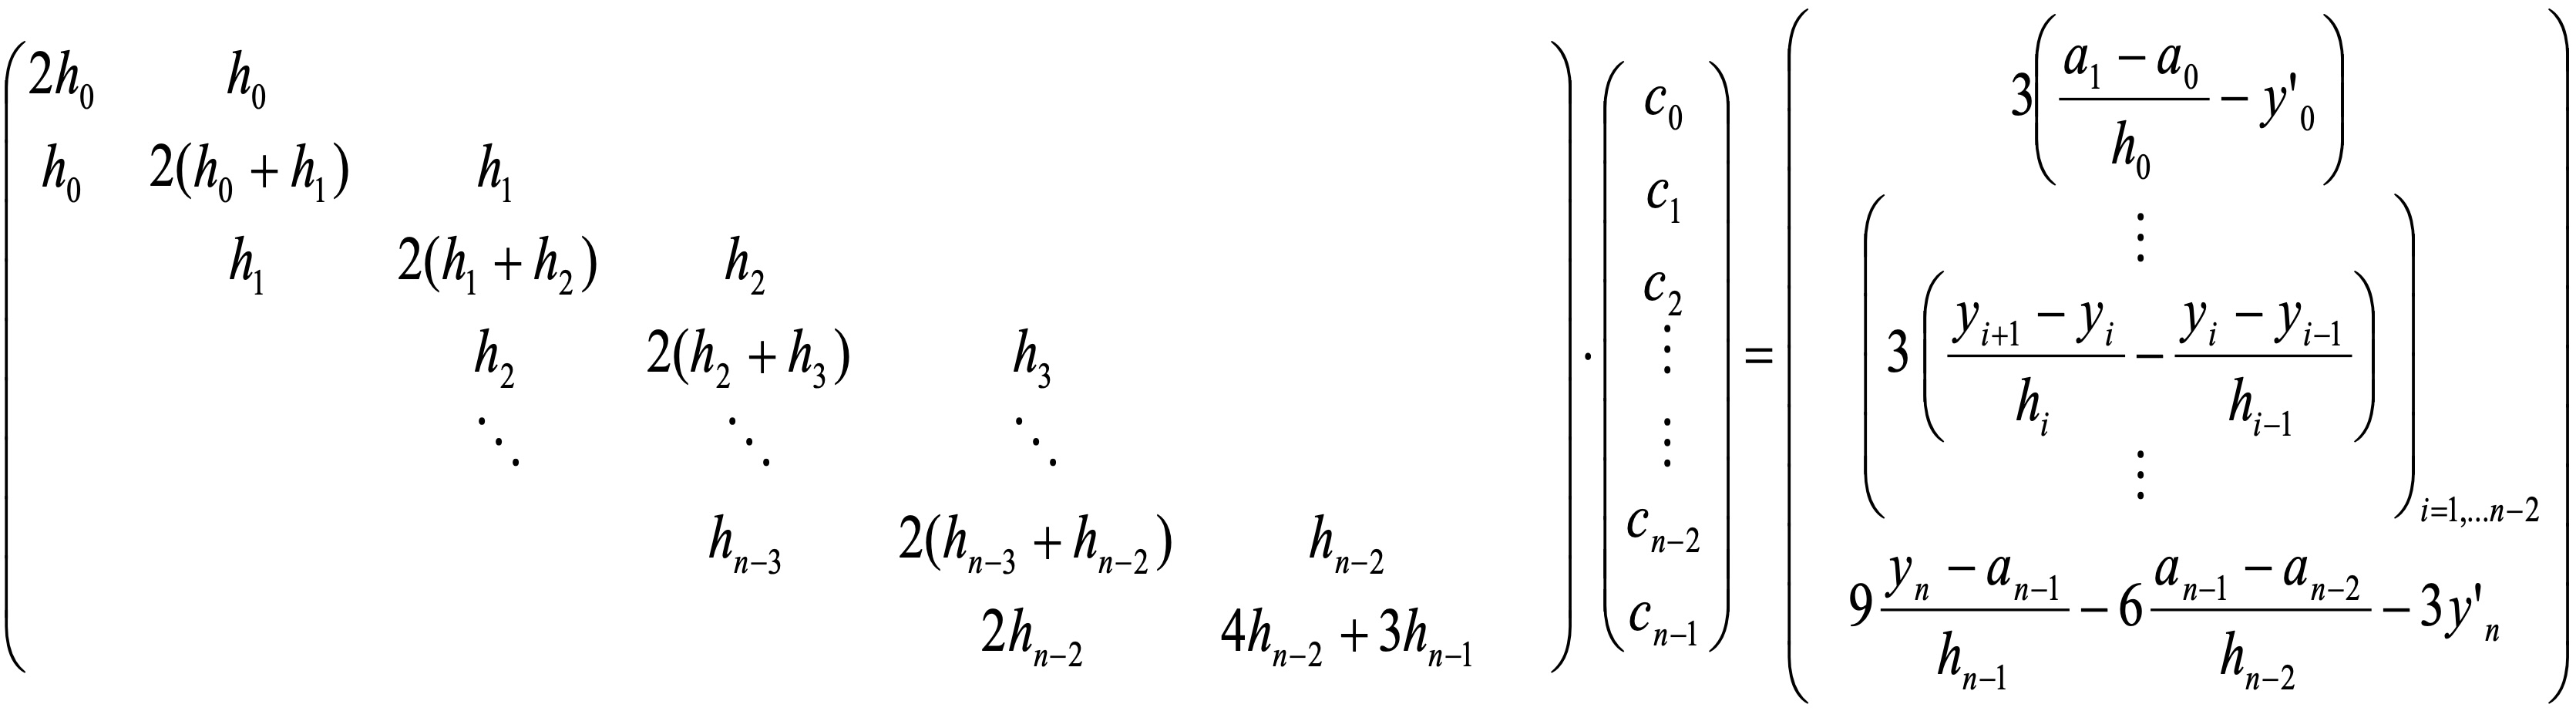
\includegraphics[width=\columnwidth]{images/clamped}}

From (\ref{spline-d}) we get $d_0,\ldots,d_{n-2}$,
from (\ref{spline-b}) we get $b_0,\ldots,b_{n-2}$ and $b_{n-1}$ from (\ref{spline-bn})
and finally $d_{n-1}$ from (\ref{spline-dn}).

\subsection{Error Formulas}
\begin{align*}
    |y(x)-S(x)| & \leq\max\frac{|y^{(4)}(x)|}{4!}\frac{5H^4}{16} = \max |y^{(4)}(x)|\frac{5}{384}H^4 \\
    |y'(x)-S'(x)| & \leq\max\frac{|y^{(4)}(x)|}{4!}H^3 = \max |y^{(4)}(x)|\frac{1}{24}H^3 \\
    |y''(x)-S''(x)| & \leq\max|y^{(4)}(x)|\frac{3}{8}H^2 \\
    & {\color{gray} x\in [x_0,x_n], H = \max_{i=0,\ldots,n-1}h_i}
\end{align*}

